\begin{apendicesenv}
\partapendices

\chapter{Cronograma Detalhado}
\label{schedule_ap}

Para evitar poluição visual no relatório, foram feitas duas versões do cronograma.
Dentro do relatório foi incluída uma versão simplificado do mesmo, sem o detalhamento de todas as atividades.
As figuras seguintes mostram o cronograma detalhado.

\begin{figure}[!htbp]
  \centering
  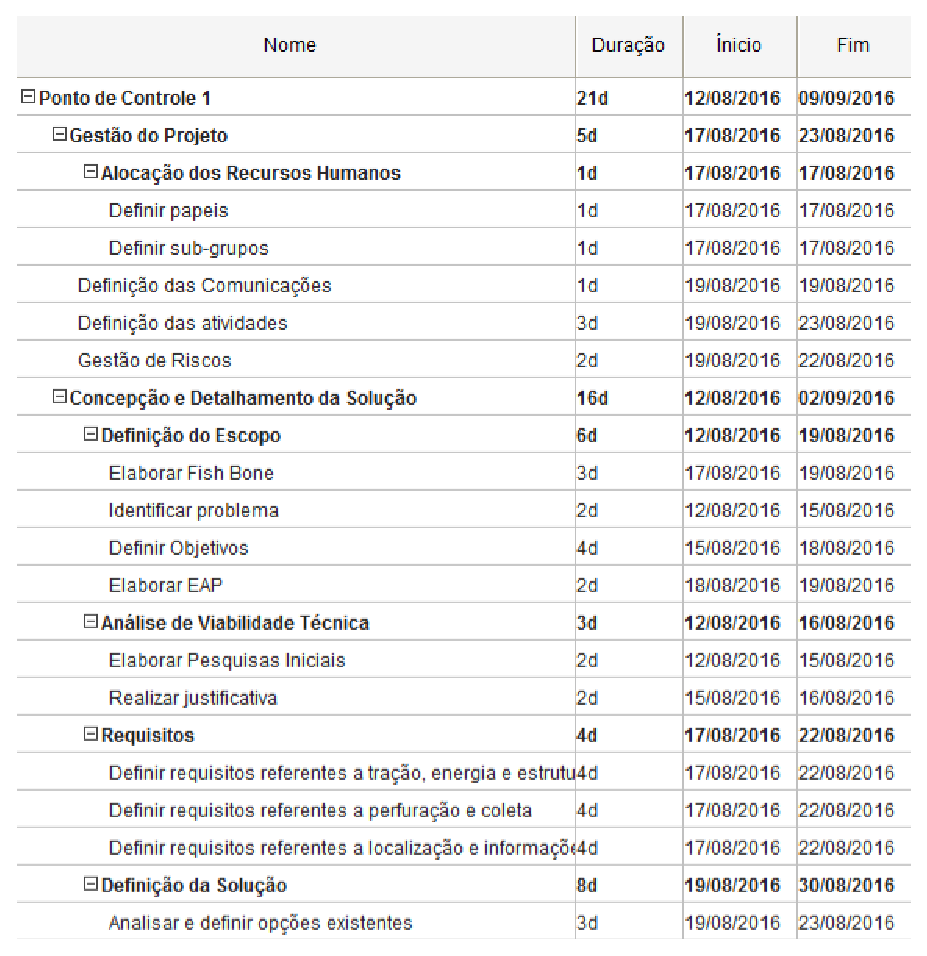
\includegraphics[width=\textwidth]{figuras/cronograma_det_1.eps}
  \caption{Cronograma de Atividades detalhado (parte 1). Fonte: autores.}
  \label{fig:cron_d1}
\end{figure}

\vfill
\pagebreak

\begin{figure}[!htbp]
  \centering
  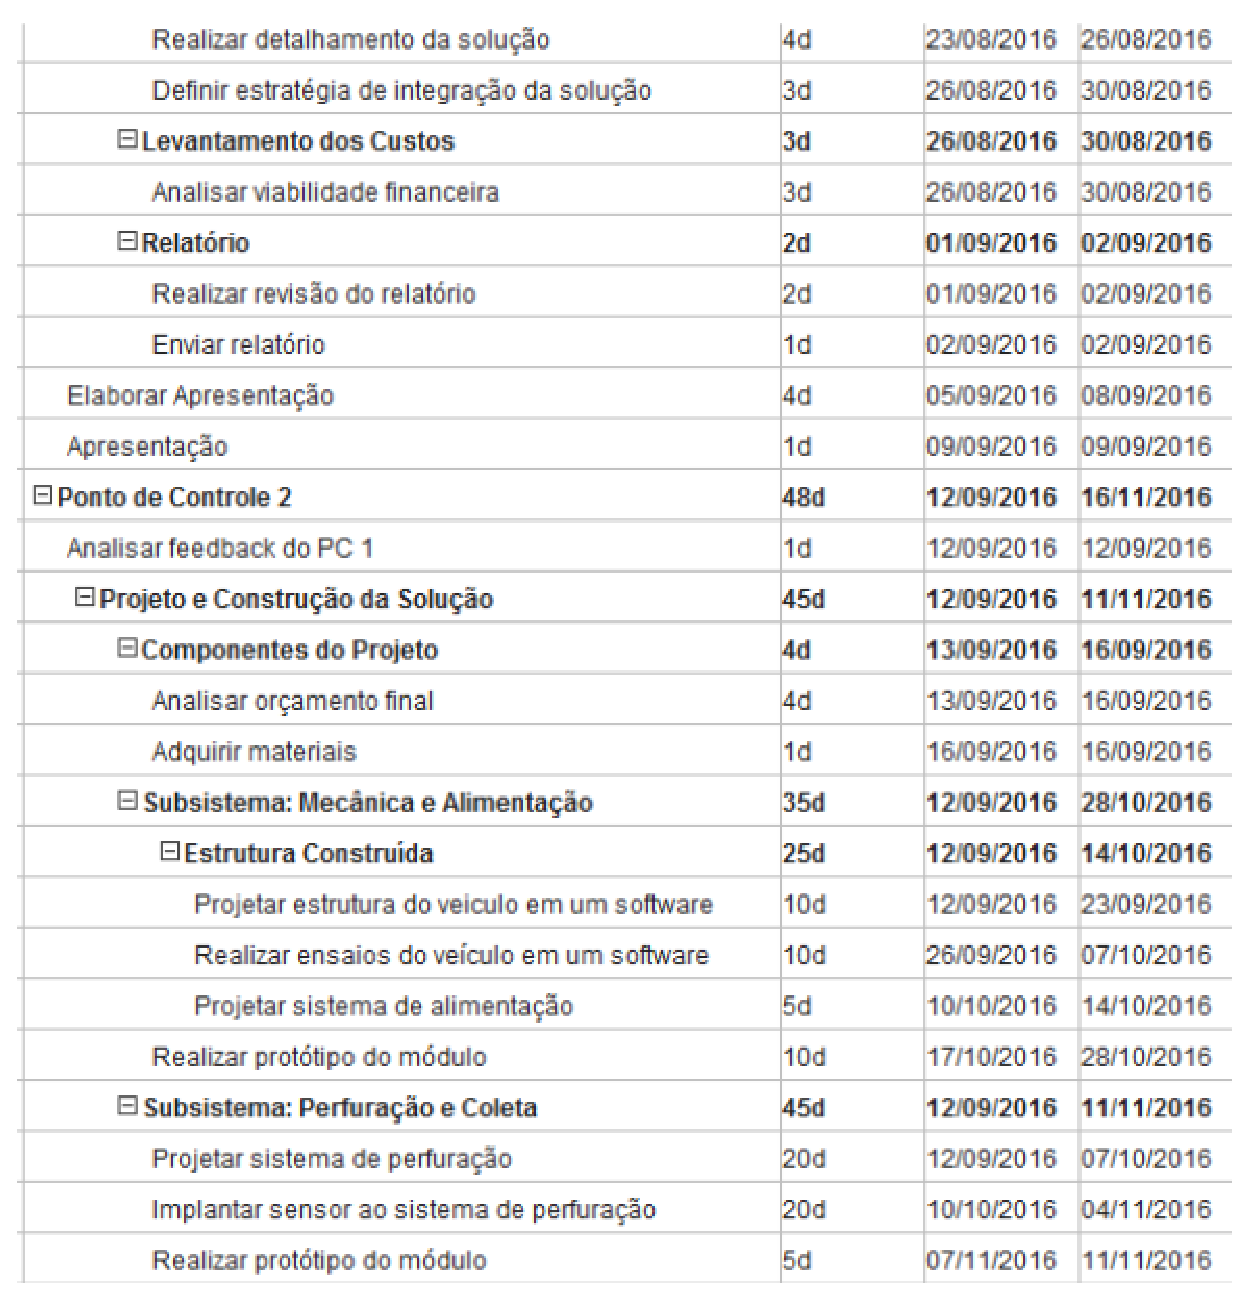
\includegraphics[width=\textwidth]{figuras/cronograma_det_2.eps}
  \caption{Cronograma de Atividades detalhado (parte 2). Fonte: autores.}
  \label{fig:cron_d2}
\end{figure}

\vfill
\pagebreak

\begin{figure}[!htbp]
  \centering
  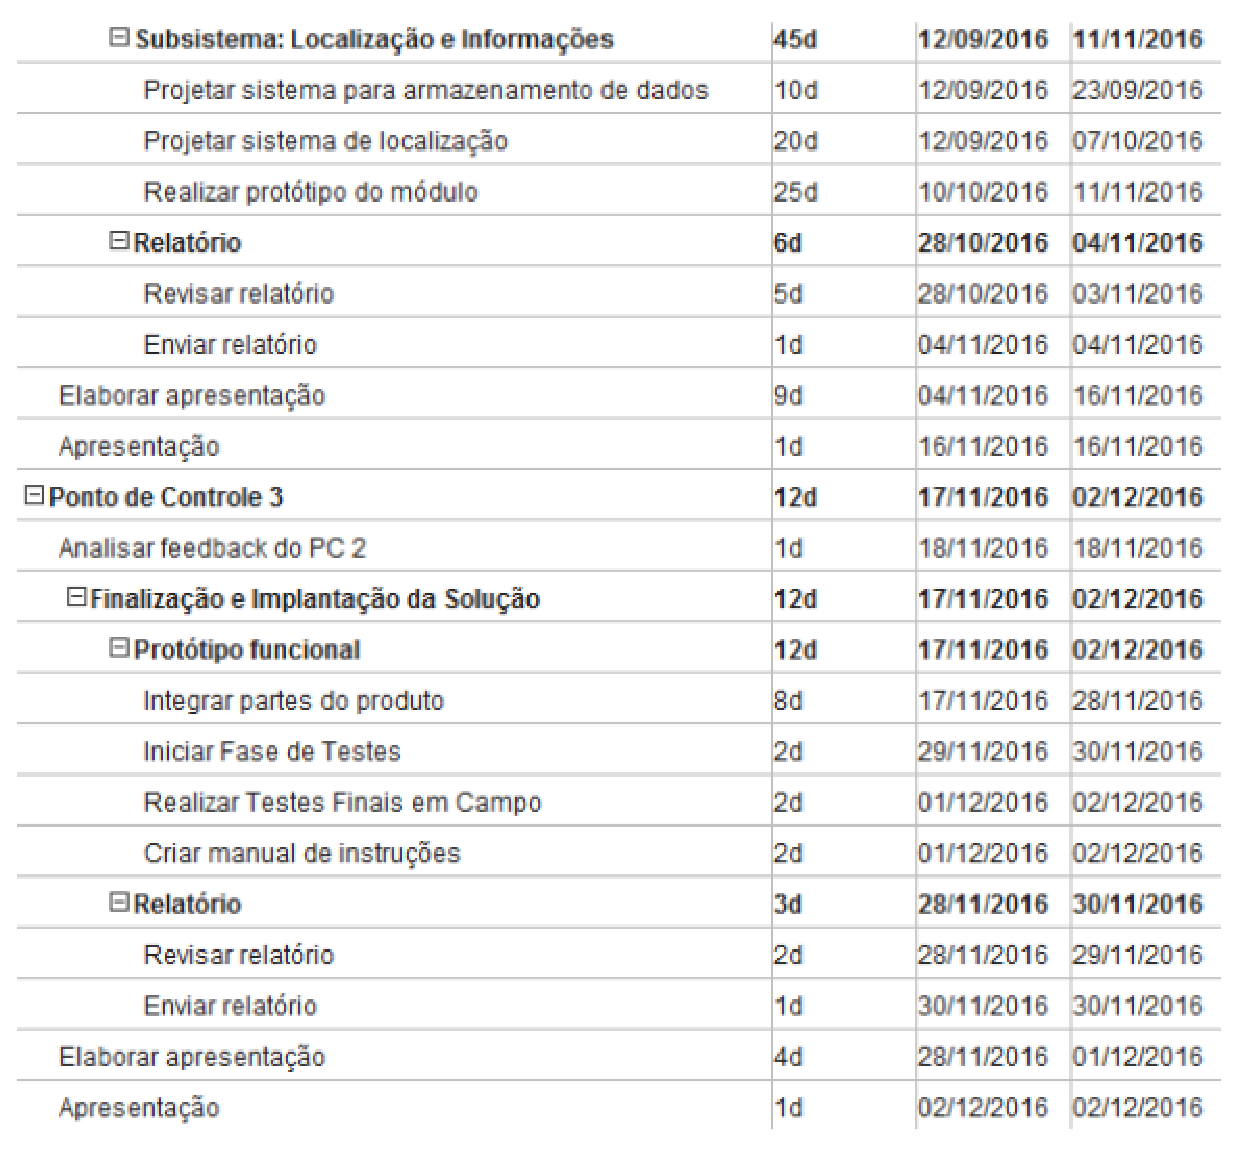
\includegraphics[width=\textwidth]{figuras/cronograma_det_3.eps}
  \caption{Cronograma de Atividades detalhado (parte 3). Fonte: autores.}
  \label{fig:cron_d3}
\end{figure}

\chapter{Desenhos Técnicos da Estrutura}

\begin{figure}[!htbp]
	\centering
	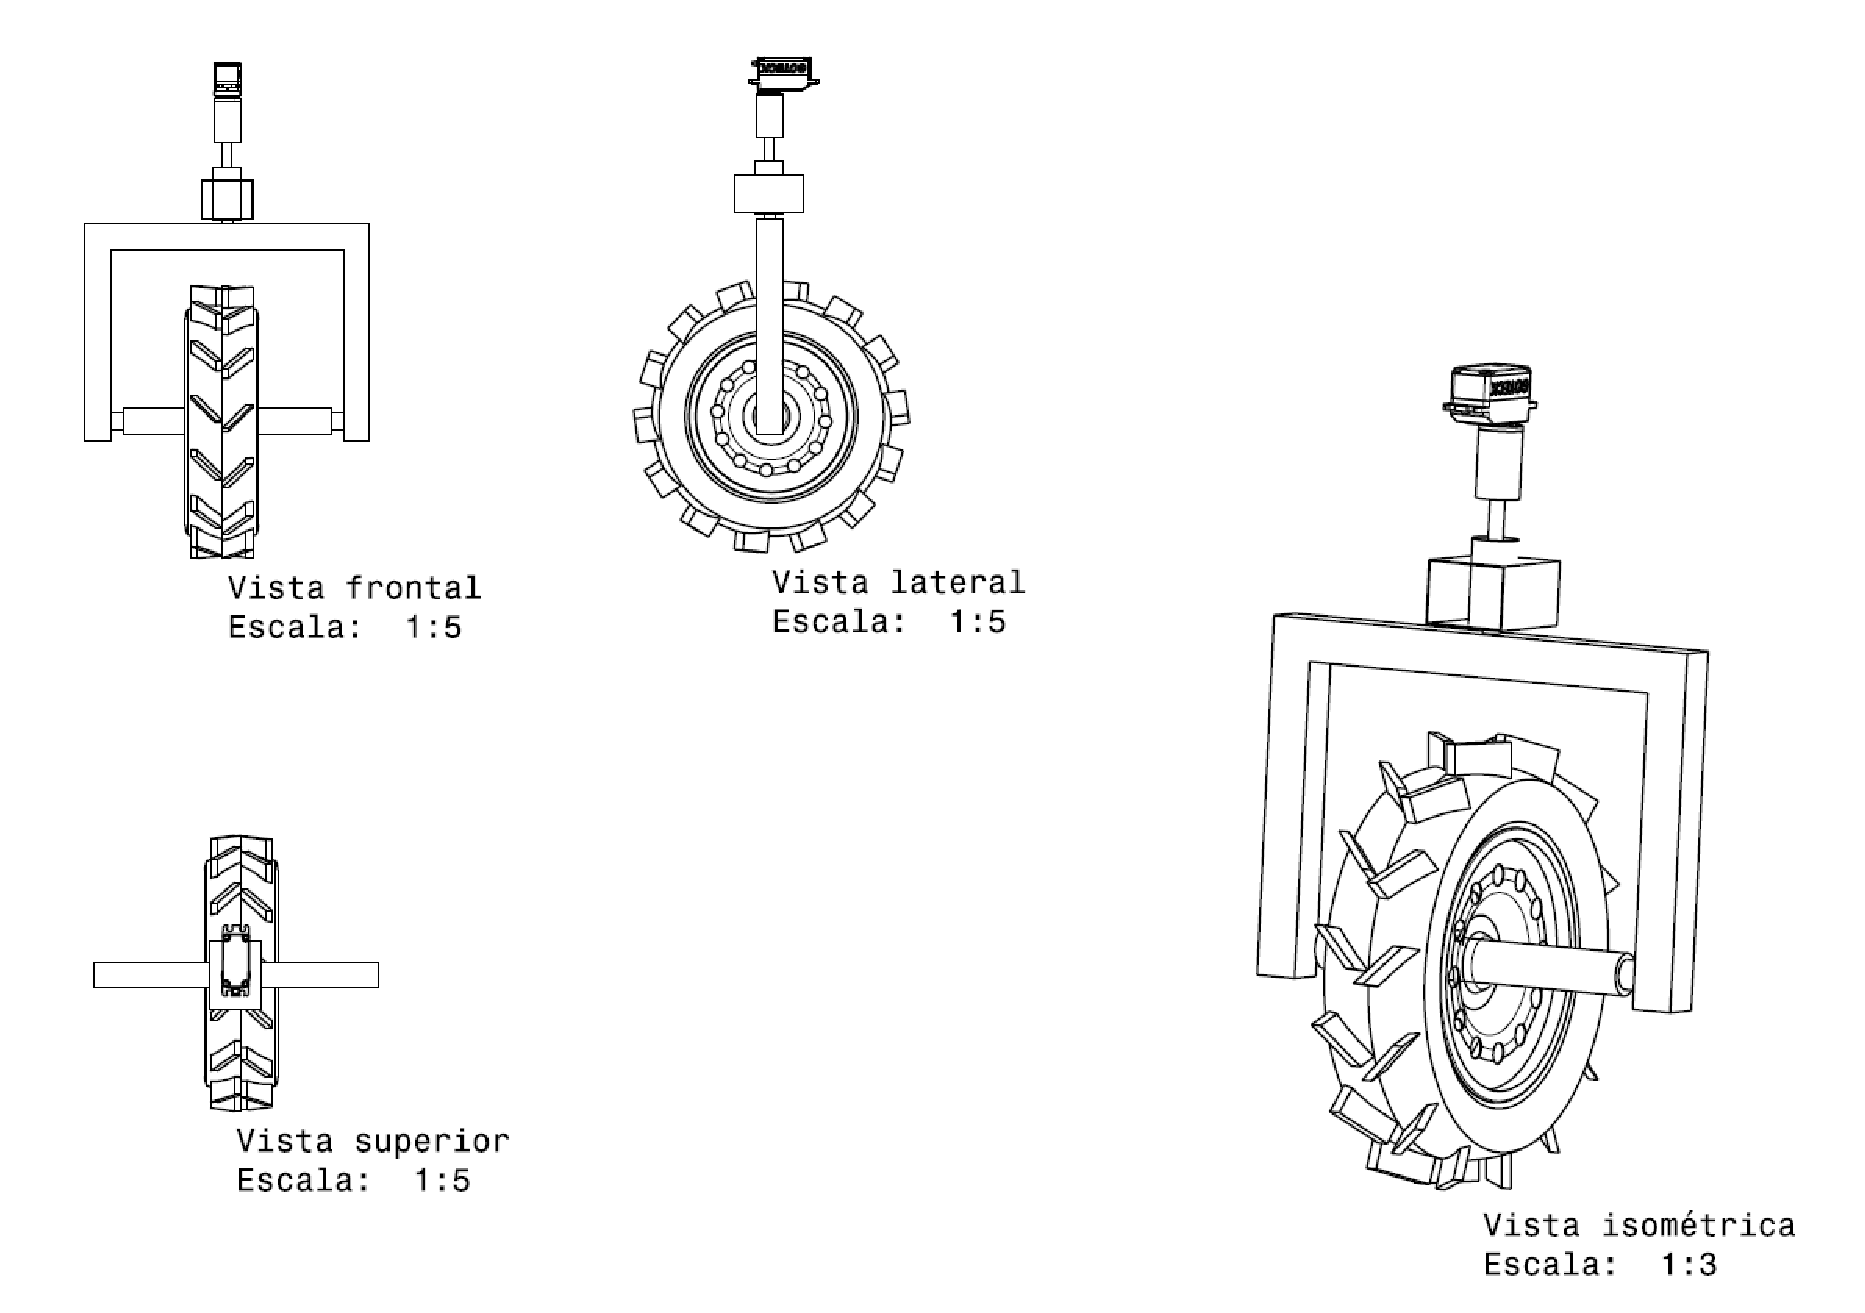
\includegraphics[width=\textwidth]{figuras/dt_direcao1.eps}
	\caption{Vistas frontal, lateral e superior da estrutura da direção}
\end{figure}

\begin{figure}[!htbp]
	\centering
	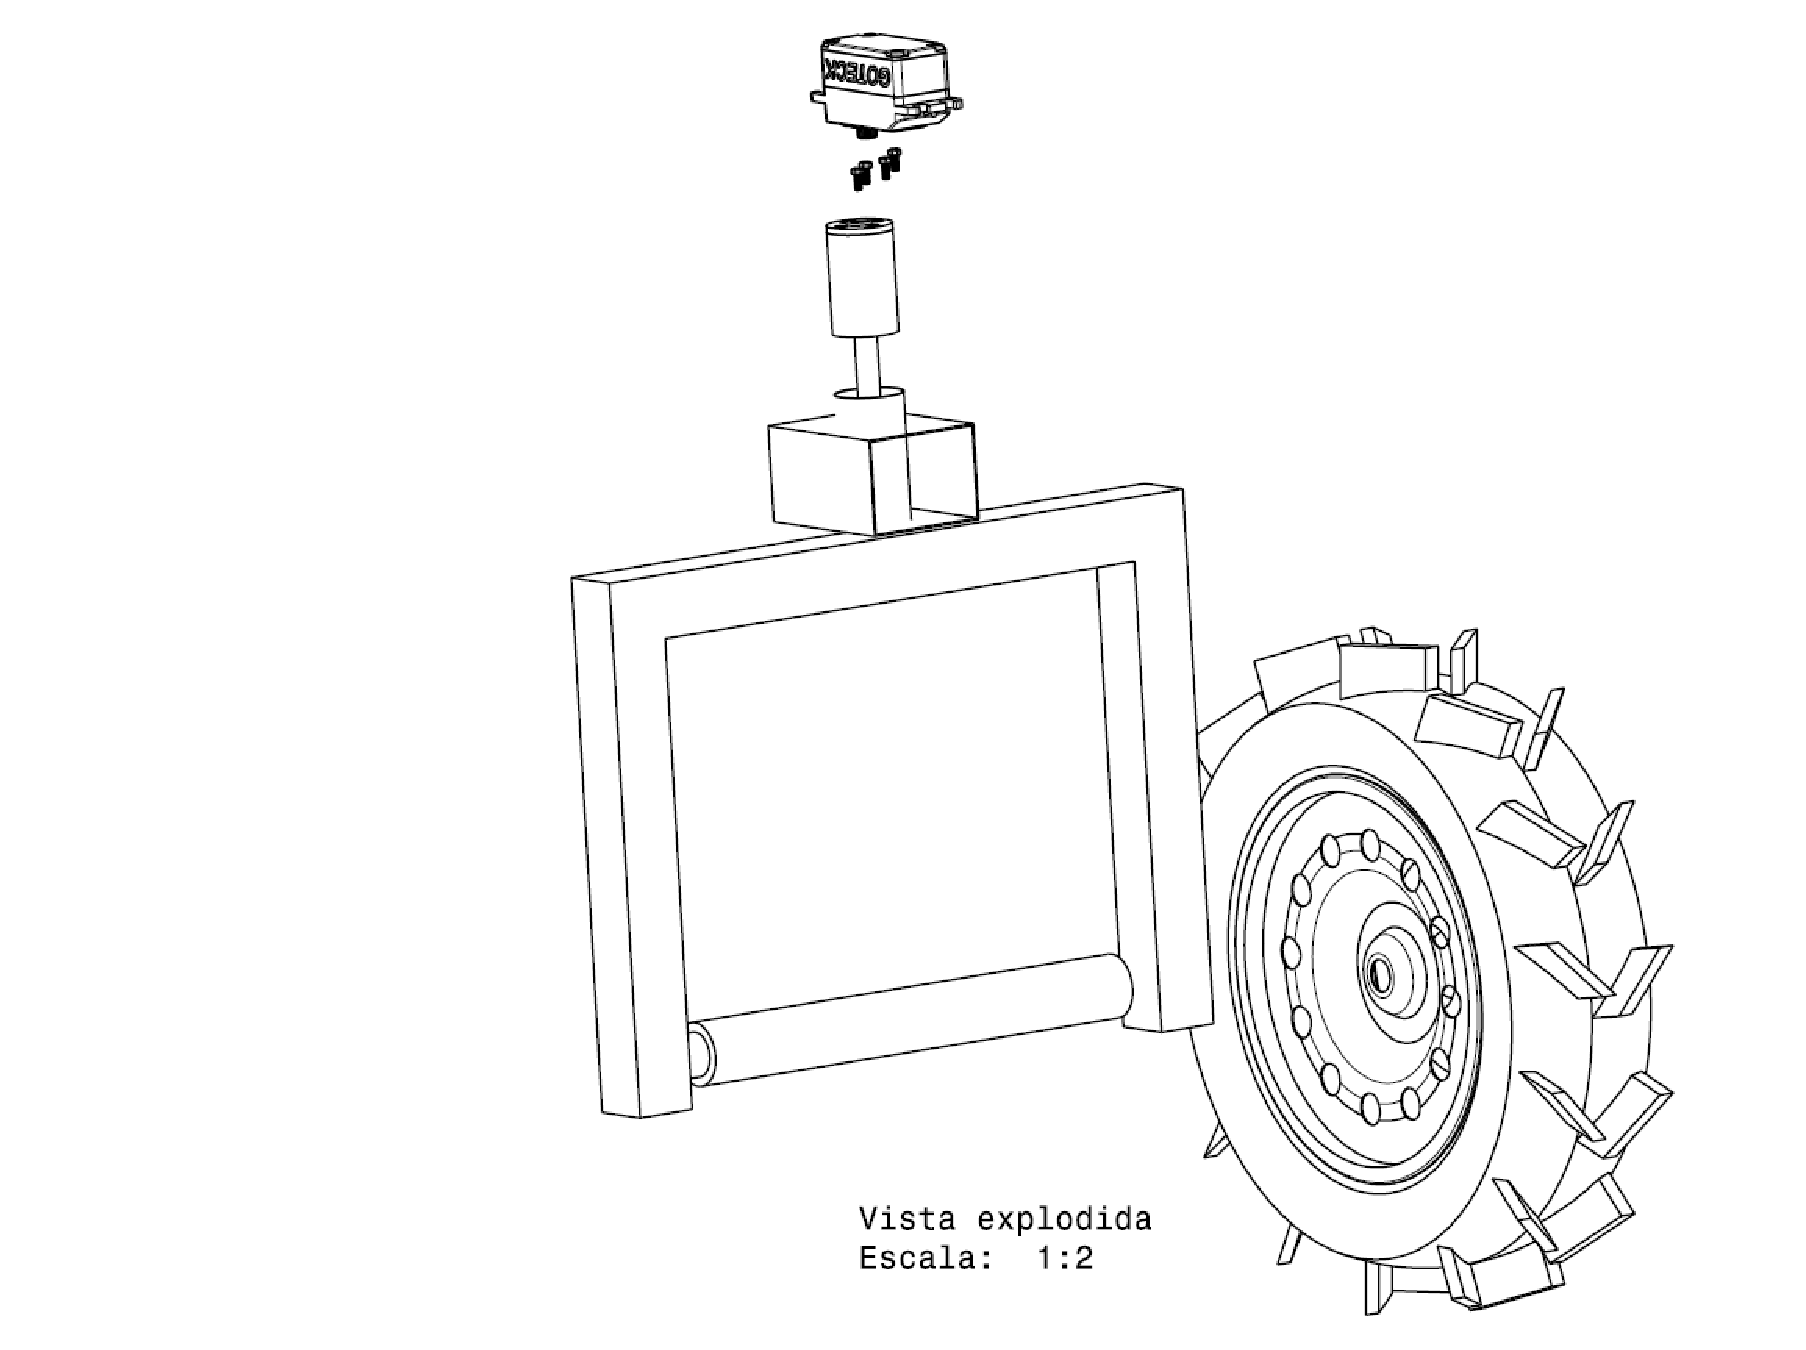
\includegraphics[width=\textwidth]{figuras/dt_direcao2.eps}
	\caption{Vista explodida do sistema de direção}
\end{figure}

\begin{figure}[!htbp]
	\centering
	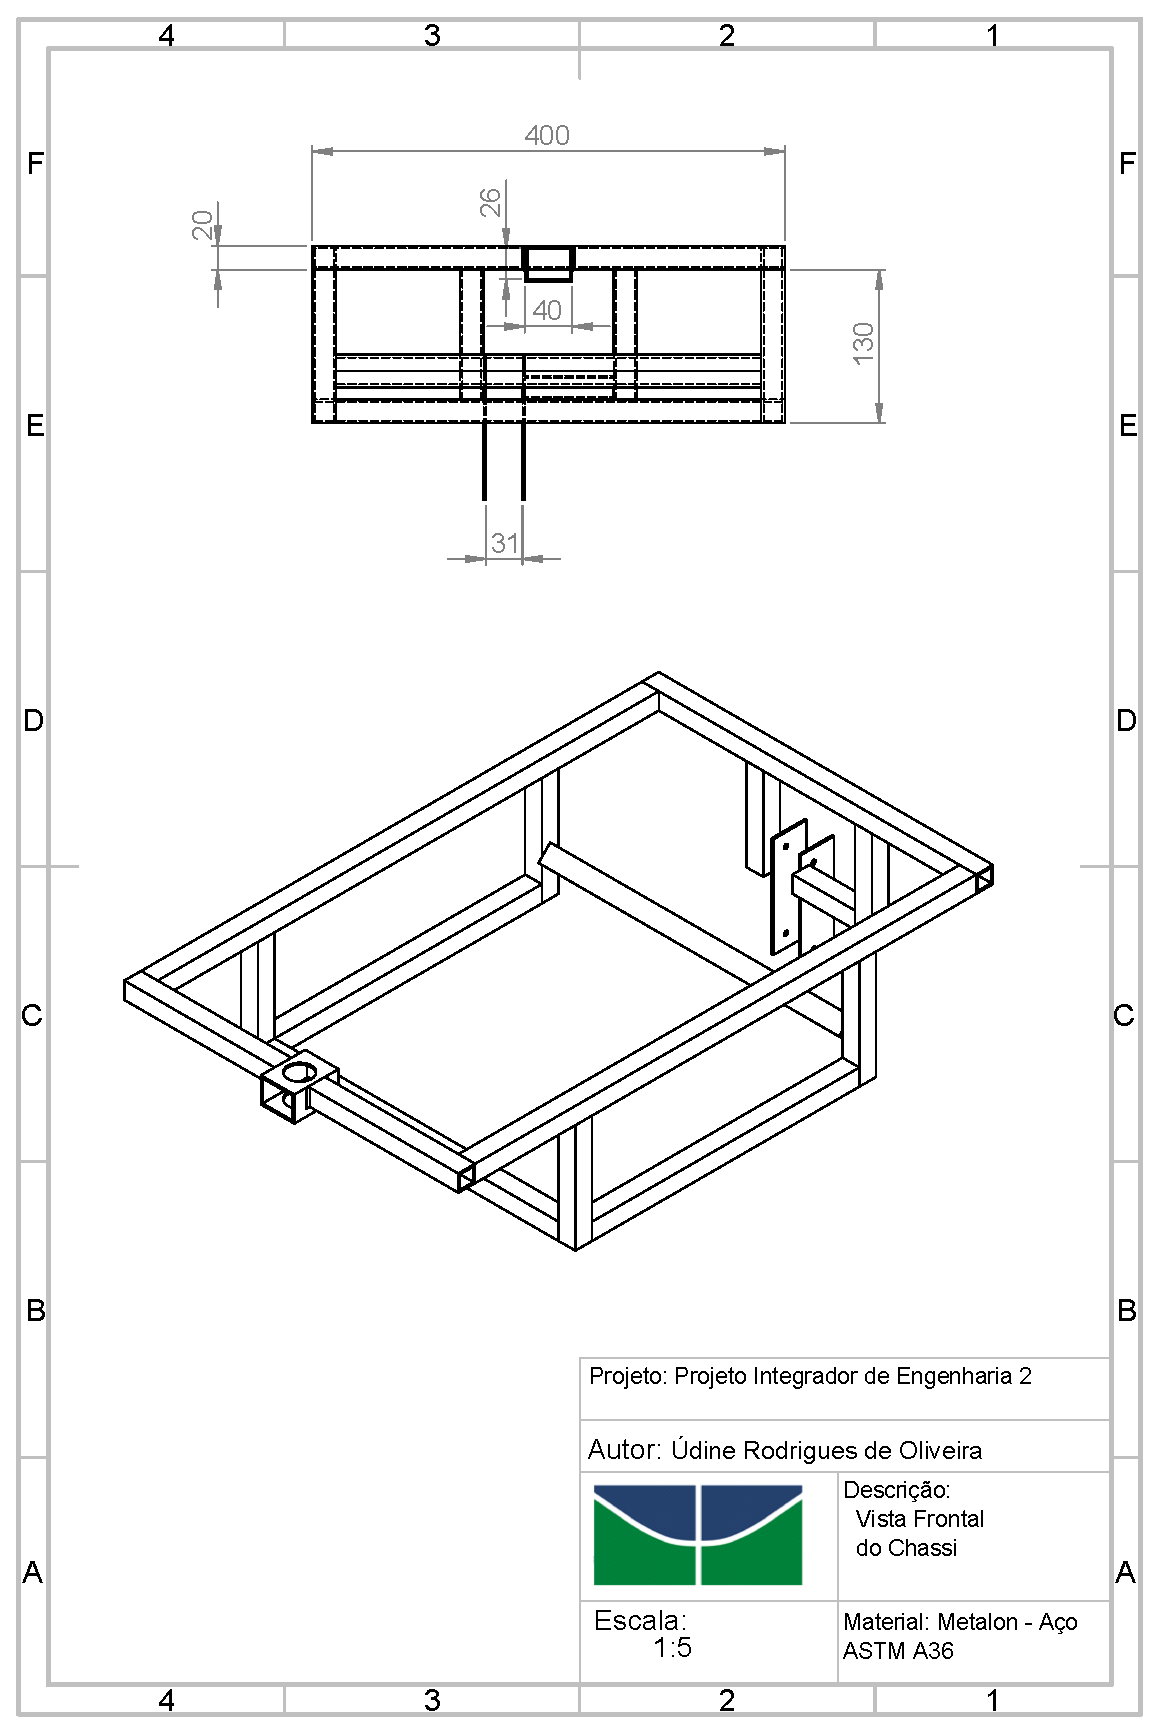
\includegraphics[width=\textwidth]{figuras/chassi_frontal.eps}
	\caption{Desenho técnico da vista frontal do chassi}
\end{figure}

\begin{figure}[!htbp]
	\centering
	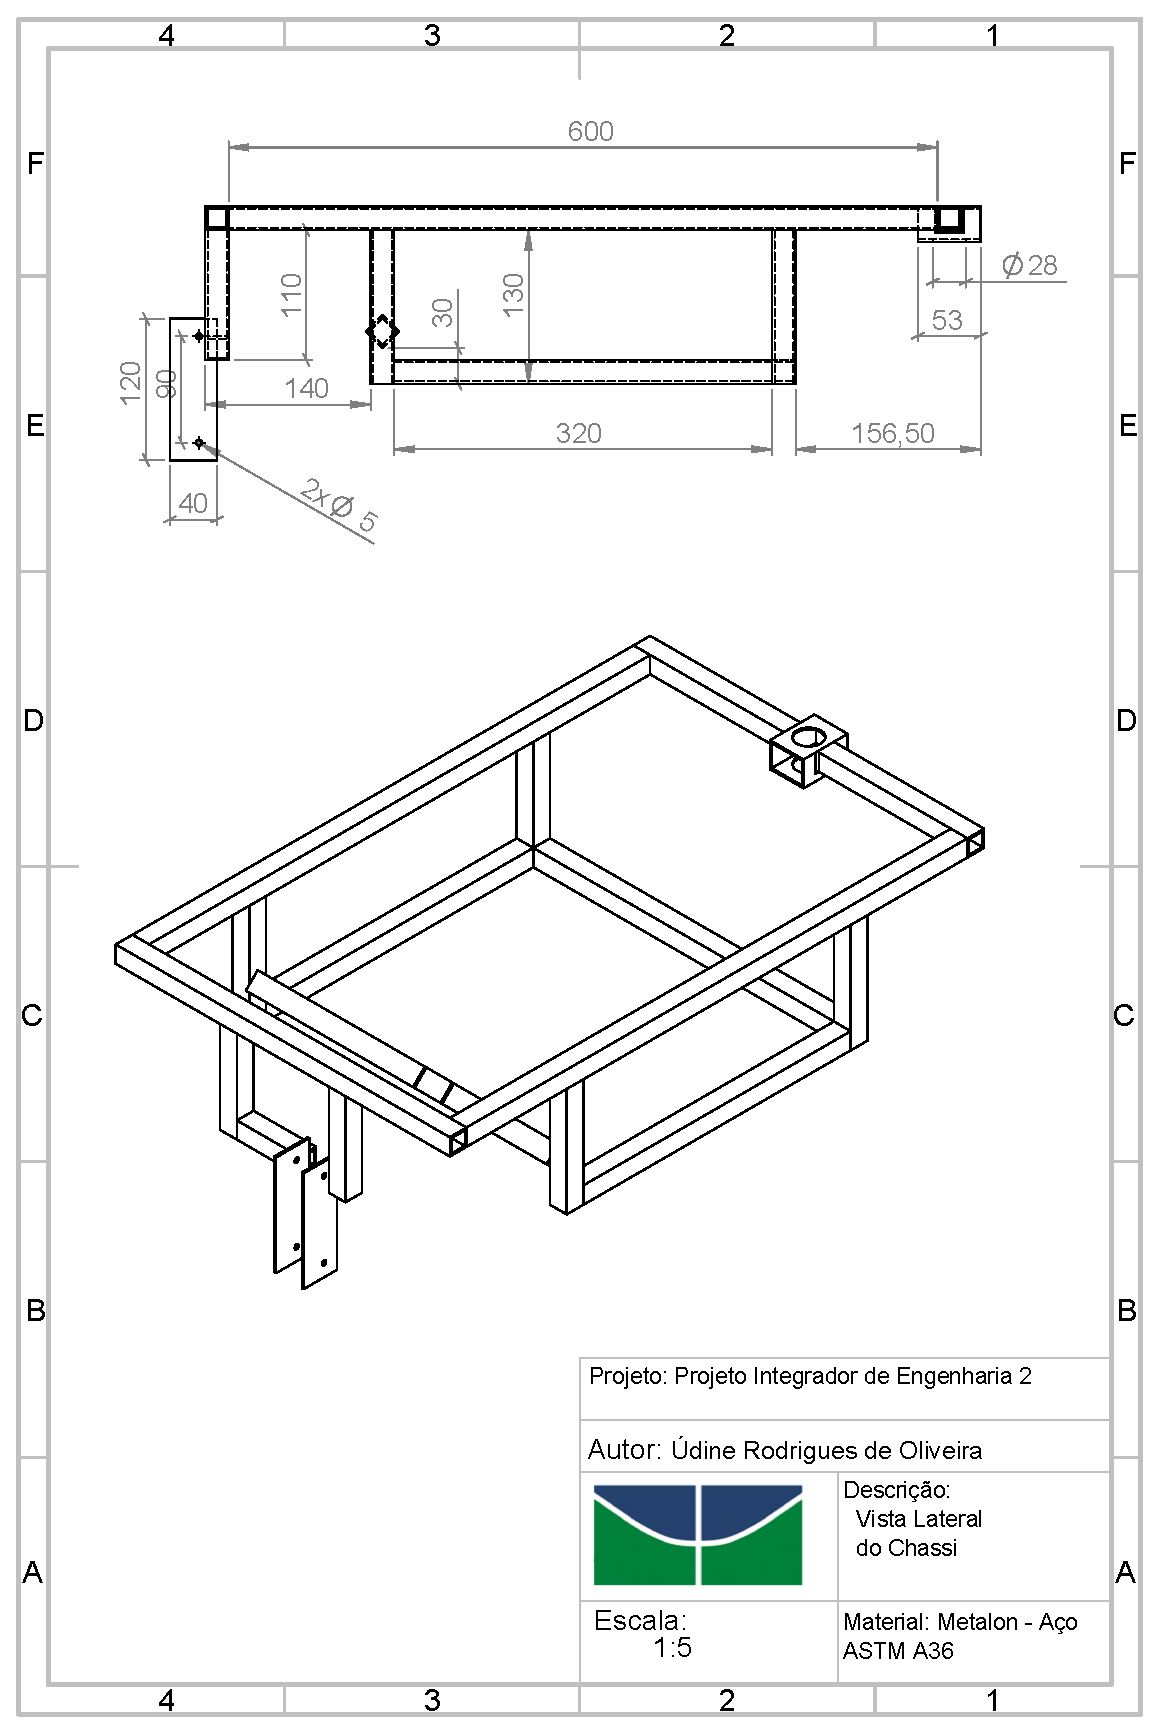
\includegraphics[width=\textwidth]{figuras/chassi_lateral.eps}
	\caption{Desenho técnico da lateral frontal do chassi}
\end{figure}

\begin{figure}[!htbp]
	\centering
	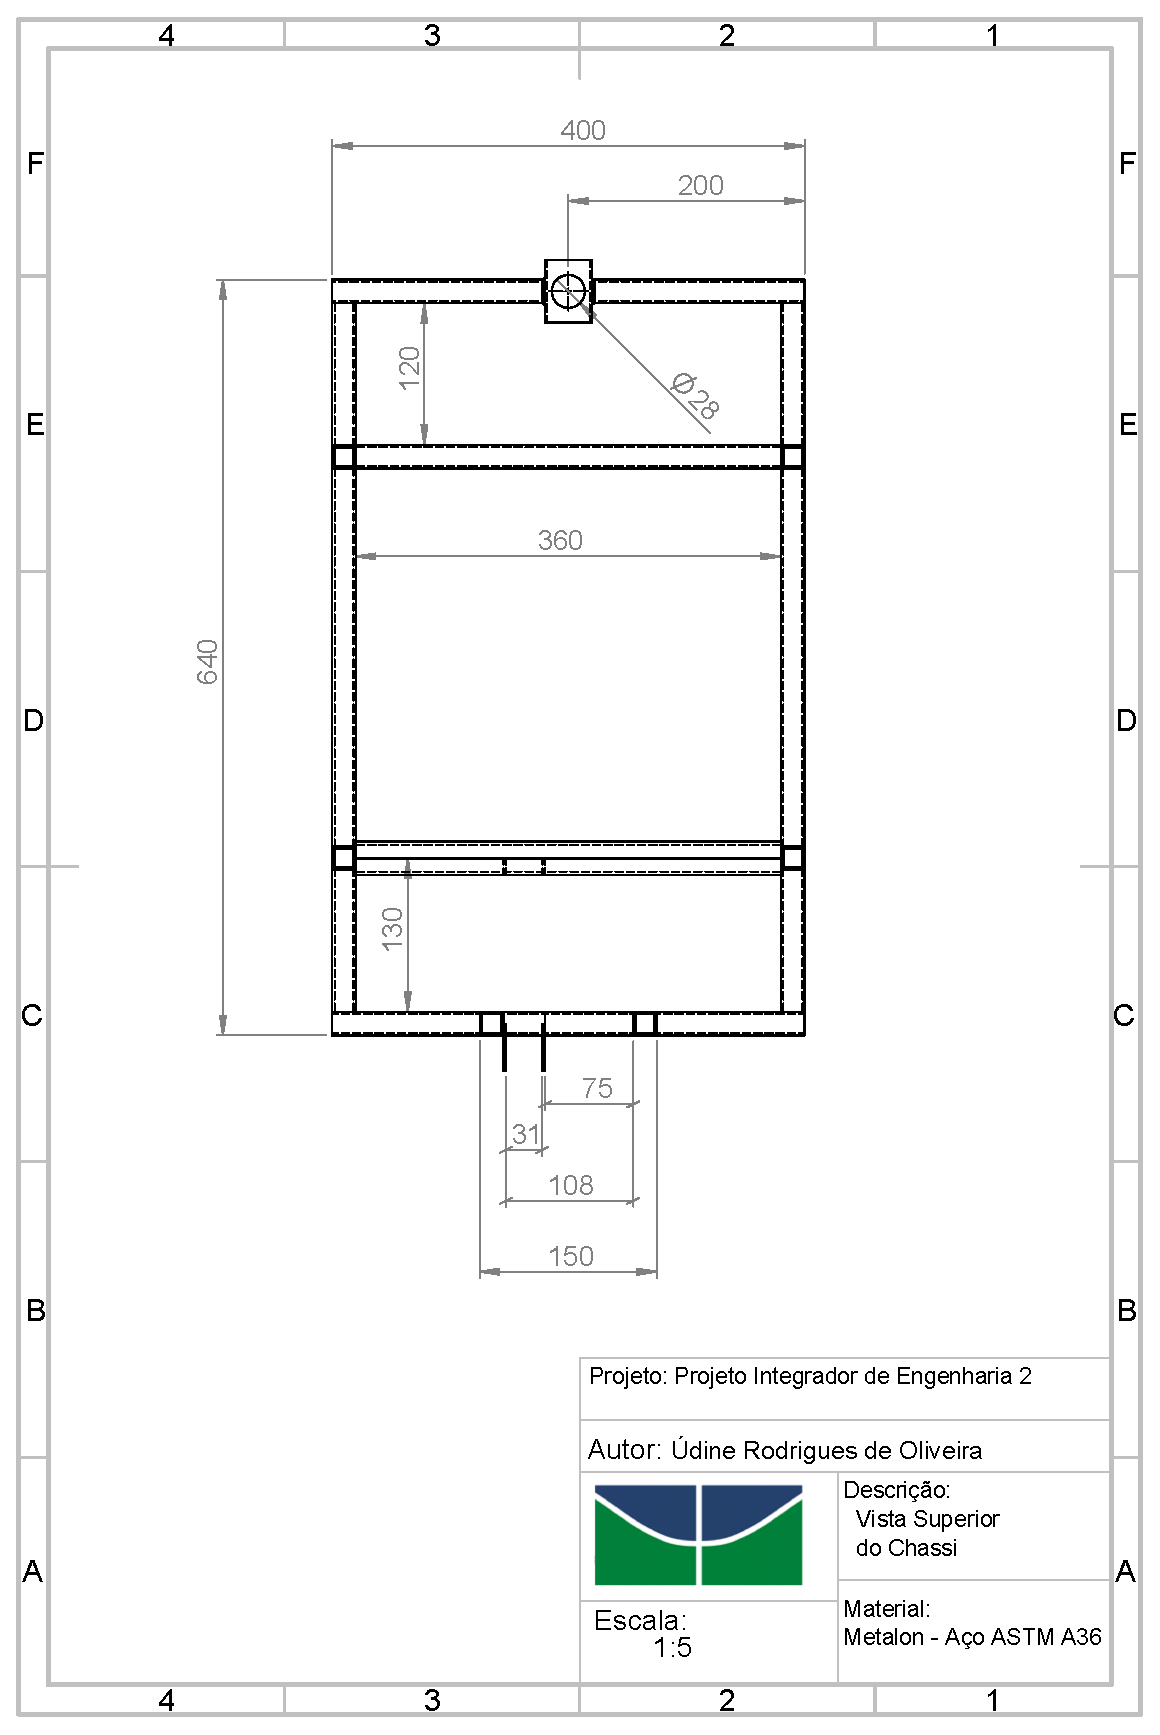
\includegraphics[width=\textwidth]{figuras/chassi_superior.eps}
	\caption{Desenho técnico da vista superior do chassi}
\end{figure}

\end{apendicesenv}
